% ------------------------------------------------------------------------------
%
% PREAMBLE
%
% ------------------------------------------------------------------------------

\documentclass[12pt, titlepage]{article}


\usepackage{graphicx, amsmath, amssymb, natbib, setspace, sectsty, verbatim, 
		mathrsfs, float}
\usepackage{MnSymbol}
\usepackage{multirow}
\usepackage{bm}
\usepackage[usenames, dvipsnames]{color}
\bibpunct{(}{)}{;}{a}{}{,}
\setlength{\parindent}{3em}
%\parskip = 1.5ex
%\linespread{1.3}
%\onehalfspacing

\pdfpagewidth 8.5in
\pdfpageheight 11in
\setlength{\oddsidemargin}{0.0in} \setlength{\textwidth}{6.5in}
\setlength{\topmargin}{0.15in} \setlength{\textheight}{8.5in}
\setlength{\headheight}{0.0in} \setlength{\headsep}{0.0in}

\usepackage{/mnt/ExtraDrive1/Work/shTex/mymacros}


% ------------------------------------------------------------------------------
%
% BEGIN DOCUMENT
%
% ------------------------------------------------------------------------------

\begin{document}

\setcounter{equation}{0}
\renewcommand{\theequation}{R.\arabic{equation}}


% ------------------------------------------------------------------------------
%
%                    Section 8.8.1
%                    Seal trend data
%
% ------------------------------------------------------------------------------

{\large \flushleft \textbf{9.11.3 Moss Heavy Metal Data}}

\vspace{.3cm}

In Section 8.7.4, we used a spatial linear model for the logarithm (base $e$) of lead (Pb) concentration in tissue samples that included explanatory variables for 1) year of sample (2001 or 2006), 2) (log, base $e$) distance-from-road, and 3) side-of-road (north or south).  We fit a mean structure where the dominant effect was distance-from-road. There also appeared to be some lowering of Pb concentration in 2006 due to better coverings on trucks that transported ore on the haul road, although the P-value of 0.118 would be judged non-significant if our critical values were $\alpha = 0.05$ or $\alpha = 0.10$. 

In prior examples in this Chapter, for the wet sulfate data and harbor seals, we used kriging and spatial prediction to make maps with point-wise or polygon-wise predictions with standard errors (mean-squared prediction errors) of those predictions.  In this Section we will focus on conditional simulation for the heavy metal data.  We have 5 prediction data sets, and they are shown as stratum 1 through stratum 5 in Figure 1.8B.  Recall that the data are modeled after a log transformation, but we wish to make inferences back on the natural scale of the data.  This nonlinear back-transformation, coupled by any further computations on a whole prediction surface, complicates the construction of the covariance matrix for predictions.  Rather, we simulate a whole surface on the transformed scale, then back-transform that whole surface, and then perform further computations.  Because we simulate many equal-probable surfaces, we perform our inference \textit{after} computing on individual surfaces by using the variation among the computed values on individual surfaces.

As an example, consider whether or not there is a difference between 2001 and 2006 in each stratum for the moss heavy metal data.  First, we simulate a surface using conditional simulation, with fixed effects set at 2001 and 2006 (so we essentially simulate the surface twice, but with the same set of fixed effects and covariance parameters).  Then, we exponentiate the values comprising the surface, average the 2001 and 2006 surfaces, and then take the averaged 2001 surface minus the 2006 surface.  Trying to find the variance of this difference would be quite difficult based on our original model on the log scale.  However, using conditional simulation, we simply simulate another surface, and repeat all computations.  

For our example, we did this 500 times, and a histogram of the differences between 2001 and 2006 are shown in Figure~\ref{Fig:MossDiffHist}.  Notice that for strata 1 through 4, there is very strong evidence that Pb concentrations went down from 2001 to 2006, as all computations from 500 conditional simulation showed positive values.  To estimate P-values, we can use quantiles from the simulations.  Here, because all 500 simulations are greater than 0, we can state that P $<$ 0.002. The histograms of these differences have a Gaussian shape, so we are also justified in using a normal distribution approximation by taking the mean of differences divided by the standard deviation of the differences.  Doing so estimates that P $<$ $10^{-5}$ for all strata.  Strata 5 is a control, being far to the south from the road, and here we see a non-significant difference between 2001 and 2006.  If we order the differences, then 67 differences are less than 0 and 433 are greater than 0, so a two-tailed P-value is 2*(1 - 67/500) = 0.268.  Using the normal approximation we obtain P = 0.403.

\begin{figure}[H]
  \begin{center}
	    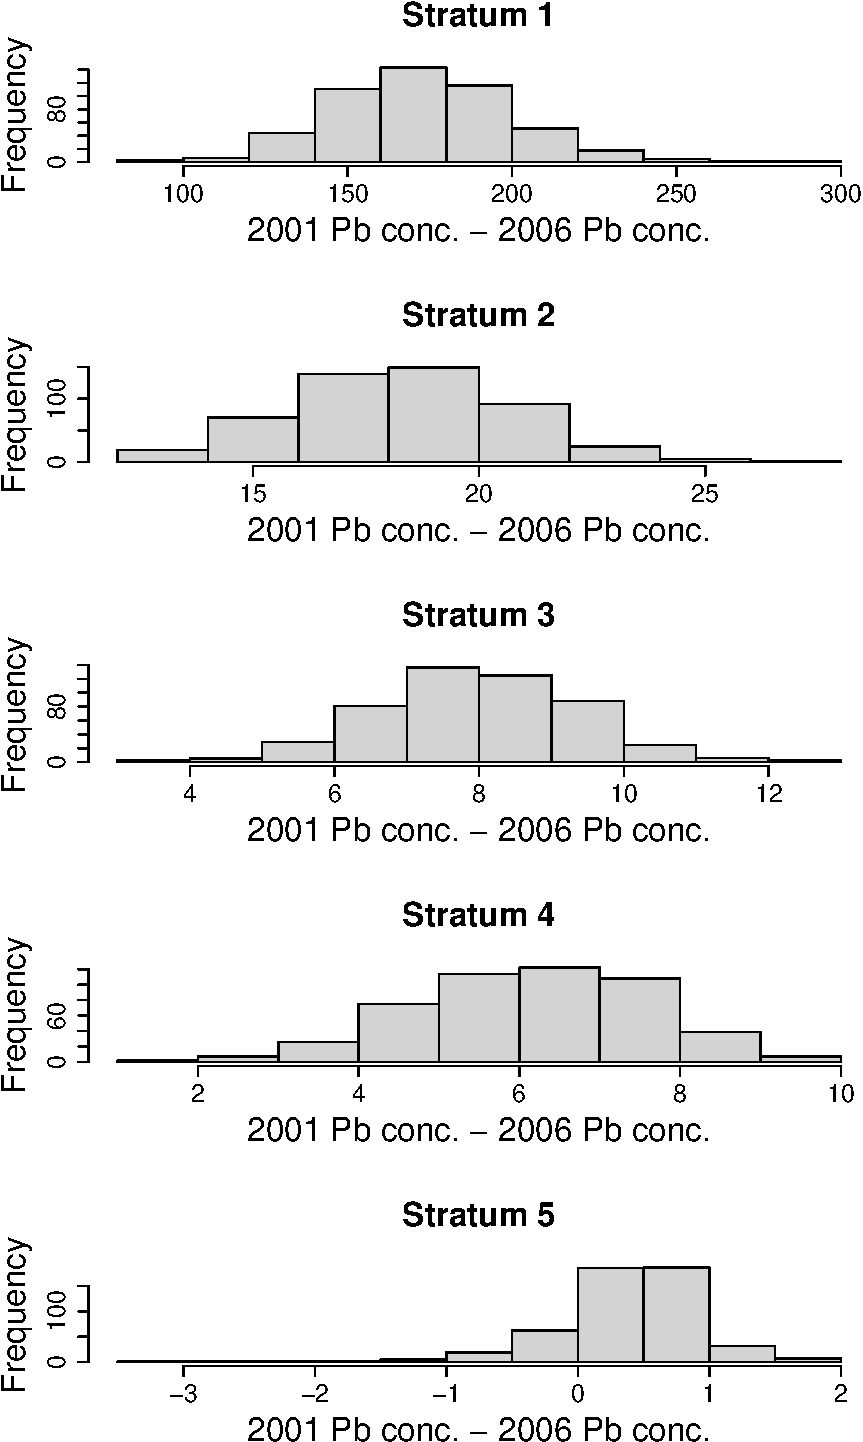
\includegraphics[width=0.5\linewidth]{figures/Moss_diffhist}
  \end{center}
  \caption{Histograms of the difference between 2001 and 2006 average Pb concentrations per stratum. \label{Fig:MossDiffHist}}
\end{figure}

Using conditional simulation, we have very strong evidence that Pb concentrations were lower in 2006 than 2001, and because the control (stratum 5) did not change significantly, we can conclude that the coverings on the trucks decreased the contamination of Pb near the haul road.  Recall that in Chapter 8, when we fit this model, while the intercepts were different between 2001 and 2006, the P-value was greater than 0.10, so that difference was not conclusive.  Why is the evidence here, using conditional simulation, so much stronger?  The reason is that in Chapter 8, we were making an inference on a mean parameter in a model, while here we are making an inference on predictions of what was actually realized in nature.  This is an important distinction that we should always keep in mind.  Do we want to make an inference on the mean of some statistical process that produced the observed data, where the data may actually be quite far from that mean, or do we want to make an inference on those realized data?  More simply, do we want to make an inference on what would happen on average if we let time start over again and our model was correct, or do want to make an inference on what actually happened.  There is no right answer, and it depends on how broadly you want your inference to apply. Notice that this may seem somewhat confusing, as we are using conditional simulation to create equal-probable surfaces, but the key word here is ``conditional,'' as those equal-probable surfaces are constrained by the observed data.

We can also use conditional simulation to make point-wise inferences.  In particular, the mean of the conditional simulation will be very similar to (essentially approximating) the kriging estimates, and the variance of the conditional simulations, point-wise, will be very similar to the kriging variance.  However, conditional simulation can be useful when our point-wise inferences are non-linear.  In our moss heavy metal example, we modeled the data on the log scale.  In the original paper by \citet{NeitlichEtAl2017Trendsspatialpatterns}, the authors were interested in maps that showed where the changes from 2001 to 2006 were highest, and the size of these changes.  The data needed to go back to the original scale of the data, and the proportional (or percent) change computed.  Thus, if $\tilde{u}_{year}$ is the prediction for the $u$th location for $year \in \{2001, 2006\}$ on the log scale, they wanted to predict $[\exp(\tilde{u}_{2006}) - \exp(\tilde{u}_{2001})]/\exp(\tilde{u}_{2001})$.  Creating unbiased predictions of this quantity, along with valid prediction intervals would be complicated.  One might use the delta method \citep{VerHoef2012Whoinventeddelta124}, but it may not be accurate.  Conditional simulation provides a straight-forward way to estimate the proportional change, along with prediction intervals. Let
$$
\ddot{u}^{[k]}= \frac{\exp(\tilde{u}_{2006}^{[k]}) - \exp(\tilde{u}_{2001}^{[k]})}{\exp(\tilde{u}_{2001}^{[k]})},
$$  
where ${u}_{year}^{[k]}$ is the $k$th conditional simulation for $year\in \{2001, 2006\}$.  Then an estimate of the proportional change at the $u$th location is mean of $\ddot{u}^{[k]}$ and prediction intervals can be obtained from the quantiles of $\{\ddot{u}^{[k]};k = 1, 2, \ldots, K\}$ for $K$ conditional simulations.

We created maps of proportional change using conditional simulation for the moss heavy metal data (Figure~\ref{Fig:MossDiffMaps}).  In general, the proportional changes were often around a 50 \% decrease, and sometimes as much as 100 \%.  However, Figure~\ref{Fig:MossDiffMaps} also reveals that the area to the northeast, especially near the road, had higher concentrations of lead.  This may be due to effects near the mine site, rather than from the road itself.  Maps such as these help uncover further possible mitigation strategies.  The point-wise 90\% prediction bounds, taken as the 0.05\% and 0.95\% quantiles from $\{\ddot{u}^{[k]};k = 1, 2, \ldots, K\}$, show that point-wise predictions lack power to say clearly at any given point that there has been a proportional decrease, except at small areas near the road and to the southwest of the study area.

\begin{figure}[H]
  \begin{center}
	    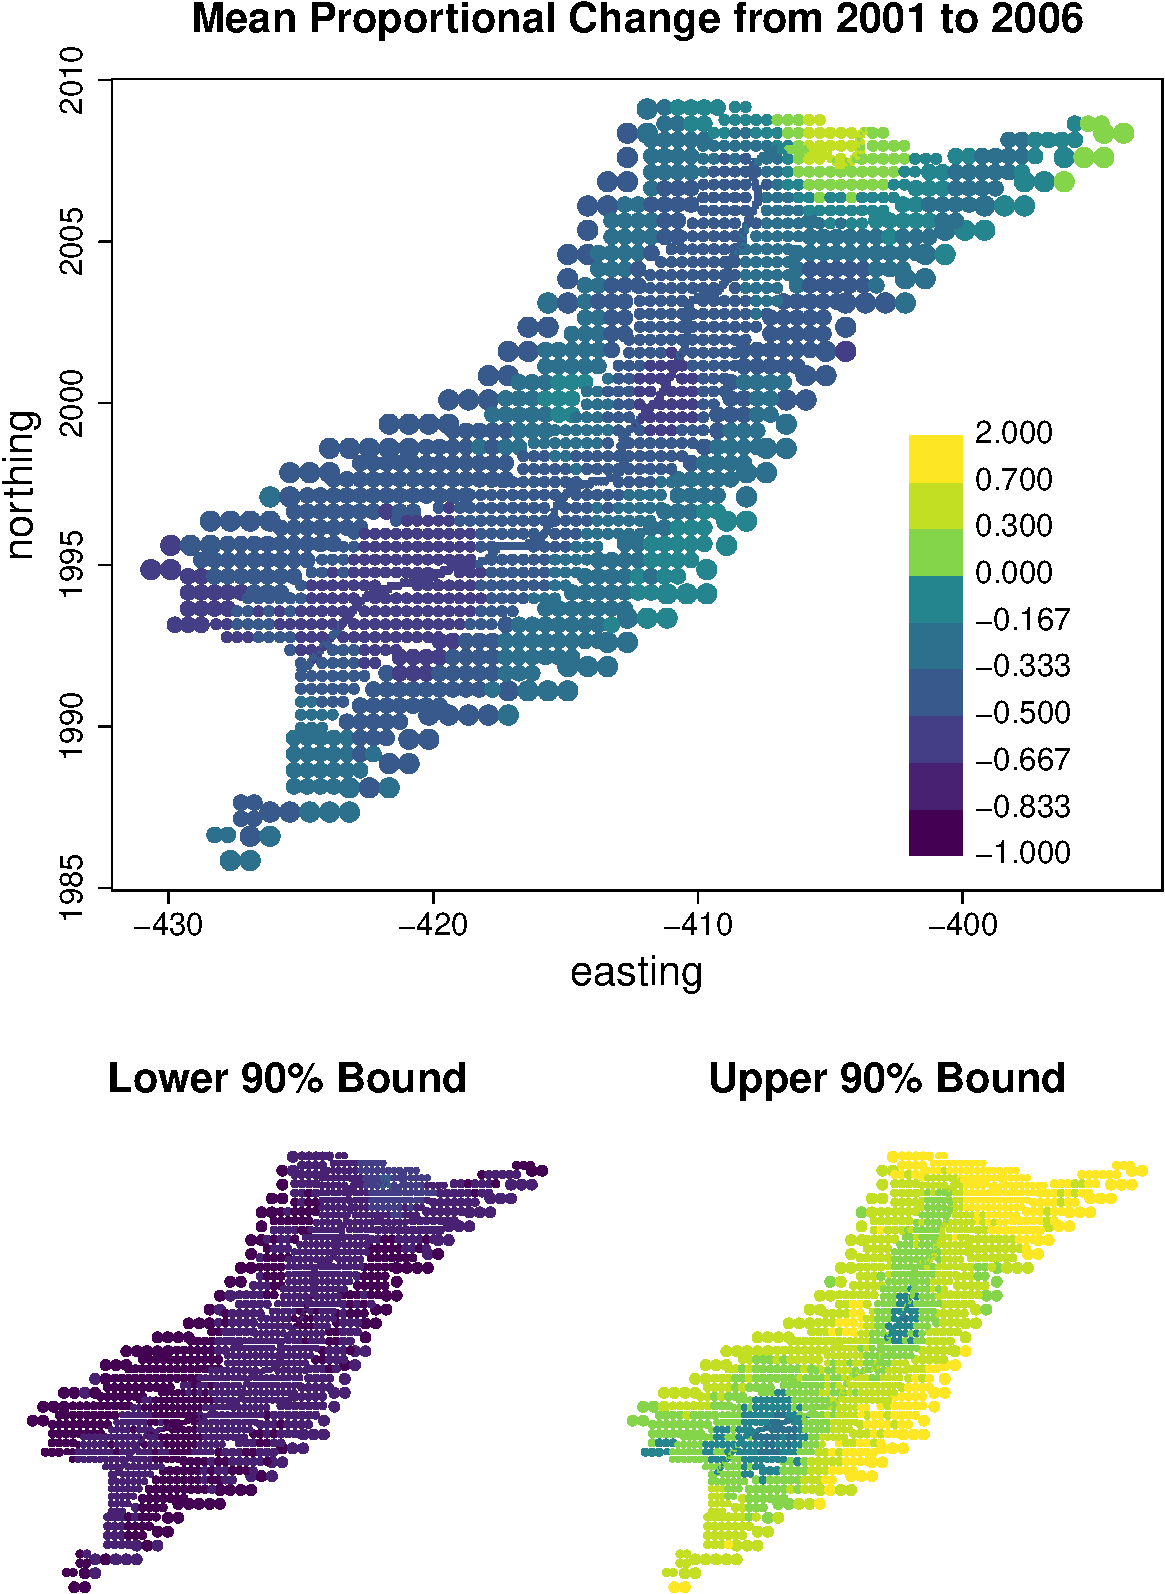
\includegraphics[width=0.8\linewidth]{figures/Moss_diffmaps}
  \end{center}
  \caption{Predicted proportional change, using conditional simulation, from 2001 to 2006 for each prediction location. \label{Fig:MossDiffMaps}}
\end{figure}

\newpage{}
When working with environmental data, a common goal is to estimate the area above a threshold.  For example, environmental law, or some other decision process, has determined that pollutants or other measured variables require action if they exceed a critical threshold.  Generally, such action is costly, so the cost of the action needs to be evaluated.  The cost may be proportional to the area above a threshold, so we need to estimate that area, and we also need to know the uncertainty, as the minimum and maximum costs are important in any decision.  Conditional simulation is ideal for estimating these quantities, and they are nonlinear functions of whole surfaces. If $\tau$ is the stated threshold, and $\mathbf{u}^{[k]}$ is the $k$th conditional simulation of all prediction locations, then
$$
\tilde{p}^{[k]} = \frac{\mathbf{1}^{T}\mathbb{I}[\mathbf{u}^{[k]} > (\tau\mathbf{1})]}{\mathbf{1}^{T}\mathbf{1}},
$$
where $\mathbb{I}(\cdot)$ is a vector indicator function, where each element is equal to 1 if its argument is true, and otherwise it is 0, and $\mathbf{1}$ is a vector of all 1's.  Inference on proportion above a threshold is then based on $\{\tilde{p}^{[k]};k = 1, 2, \ldots, K\}$, where means, median, quantiles, standard deviation, etc., and be computed.

As an example using the moss heavy metal data, we arbitrarily set a threshold of 55 mg/kg for lead concentration, and then estimated the proportion of prediction locations that exceeded this threshold.  To compute area above a threshold, we would simply take the proportion above the threshold times the total area, so he we only present the proportion above the threshold.  Table~\ref{tab:PAboveThresh} shows that in 2001 the estimated proportion of lead concentration above 55 mg/kg was 0.984 in stratum 1, with a 95\% interval ranging from 0.963 to 0.996.  The proportion was clearly and significantly lowered by 2006.  Stratum 1 is the area very close to the road, so let us concentrate on strata 2 and 3, as these are the areas of greatest concern.  Looking at stratum 2, the area above the threshold was decreased to about 1/4 of the area from 2001 to 2006, in both the estimates and bounds.  This reduction in contaminated area can be judged against the cost of adding better, more expensive coverings, to trucks hauling the ore on the road.  Moreover, looking at stratum 3, the coverings can be judged as a complete success between 2001 and 2006, and, again, the cost can be evaluated against that success.

\begin{table}[h] 
				\caption{Estimated proportion of strata 1 through 3 above 55 mg/kg concentration of lead using conditional simulation. \label{tab:PAboveThresh}}
\begin{center}
\begin{tabular}{c|rrr|rrr|}
  \hline
  \hline{}
  {} & \multicolumn{3}{c|}{2001} & \multicolumn{3}{c|}{2006} \\
  Stratum & Lower95 & Median & Upper95 & Lower95 & Median & Upper95 \\
	\hline
  \hline
	1 & 0.963 & 0.984 & 0.996 & 0.735 & 0.821 & 0.884 \\ 
  2 & 0.169 & 0.213 & 0.267 & 0.030 & 0.050 & 0.080 \\ 
  3 & 0.007 & 0.017 & 0.036 & 0.000 & 0.000 & 0.010 \\ 
  \hline
	\hline
\end{tabular}
\end{center}
\end{table}

With these examples, we have shown that conditional simulation is an important prediction method, in addition to kriging, when working with environmental data.  Many problems require functions that are computations of whole surfaces, and it is important to assess the uncertainty of those computations.  Conditional simulation provides predictions, and prediction bounds, for nonlinear functions of predictions and whole surfaces.

%%%%%%%%%%%%%%%%%%%%%%%%%%%%%%%%%%%%%%%%%%%%%%%%%%%%%%%%%%%%%%%%%%%%%%%%%%%%%%%%
%%%%%%%%%%%%%%%%%%%%%%%%%%%%%%%%%%%%%%%%%%%%%%%%%%%%%%%%%%%%%%%%%%%%%%%%%%%%%%%%                BIBLIOGRAPHY
%%%%%%%%%%%%%%%%%%%%%%%%%%%%%%%%%%%%%%%%%%%%%%%%%%%%%%%%%%%%%%%%%%%%%%%%%%%%%%%%
%%%%%%%%%%%%%%%%%%%%%%%%%%%%%%%%%%%%%%%%%%%%%%%%%%%%%%%%%%%%%%%%%%%%%%%%%%%%%%%%

%\bibliographystyle{consbiol}
\bibliographystyle{/mnt/ExtraDrive1/Work/shTex/asa}
\bibliography{DaleChap9103.bib}
%\bibliographystyle{/home/jay/Data/shTex/shTex/asa}
%\bibliography{/home/jay/Data/shTex/shTex/StatBibTex.bib}




\end{document}

